With a clear panorama of convolution and Fourier transform concepts, it is possible to enlighten the \emph{image enhancement} concept and its relevant applications to this work. Image enhancement is the process of manipulating an image in order to provide a resulting representation that is more suitable for a particular problem, e.g. an enhancement method for medical images may not be efficient for satellite images \cite{gonzalez2018digital}. Within microscopy, image enhancement is desirable due to the limited capacity of optical imaging devices and also the features of each microscopy technique, e.g. acquisition with different illumination settings, focal planes, time intervals or spectral channels; hence, enhancement algorithms for microscopy should cover all types of information \cite{wu2008microscope}. According to \citeonline{wu2008microscope}, image enhancement techniques are divided into \emph{spatial domain}, \emph{Fourier transform} and \emph{wavelet transform} methods and will be described as follows. 

The spatial domain methods are basically transforms that globally maps the gray levels of an image (or the gray levels the channels from a multichannel image, such as RGB) to their enhanced stated. Some examples are contrast stretching, which adjusts all gray levels of an image to fit among the desired range, thresholding, which applies a decision function that creates a binary image based on a preset gray level, histogram equalization, and spatial filtering. Particularly, histogram equalization and spatial filtering play an important role in this work and therefore will be explored further.

Fourier transform domain methods operate with images as a distribution of frequencies since some features are better described by it. Noise, for example, may be suppressed in a sharpening process or reduced by amplifying mid-frequency components and attenuating high-frequency ones. The Wiener Filtering process is an extensively used example of a frequency domain enhancement method that recovers a noisy signal or image based on estimations of spectral properties from the original image. Other examples of Fourier domain enhancement are band-pass filters and least-squares deconvolution applications.

Finally, the wavelet transform based methods enhance images based on Wavelet Transforms, i.e. mathematical frameworks that decompose signals and images into frequency components in different scales. Some approaches such as thresholding may be applied to wavelet coefficients, and since the output of wavelet transforms depend on the chosen wavelet function, many possible variants depend on the image features. 

\subsection{Histogram Equalization}

The image histogram is one of the simplest and most useful tools in image processing and consists of a function that summarizes the gray level content of an image in terms of a frequency distribution \cite{castleman1996digital}. The histogram equalization consists of applying a non-linear monotonic mapping to provide an approximation of a uniform distribution to the output image's histogram \cite{gonzalez2018digital}. The output histogram is a normalization of the cumulative histogram of the image, given by

\begin{equation}
\label{eqn:histogram_equalization}
hist_{equalized}(r) = \frac{L - 1}{MN} hist_{cumulative}(r),
\end{equation}

\noindent where $hist_{equalized}(r)$ and $hist_{cumulative}(r)$ are the equalized and cumulative histograms relative to a range $L$ of intensities after image quantization with $r$ values, $M \times N$ is the image resolution. Since it stems from a sum of probabilities and no new gray intensity levels should be created, the process generates fractional values that are mapped onto integers. The result of this process is contrast enhancement, which may be seen in Figure \ref{fig:histogram_equalization}:

\begin{figure}[htb]
	\centering
	\caption{\label{fig:histogram_equalization} Example of histogram equalization of dark and light images of a scene.} 
	\begin{center}
	    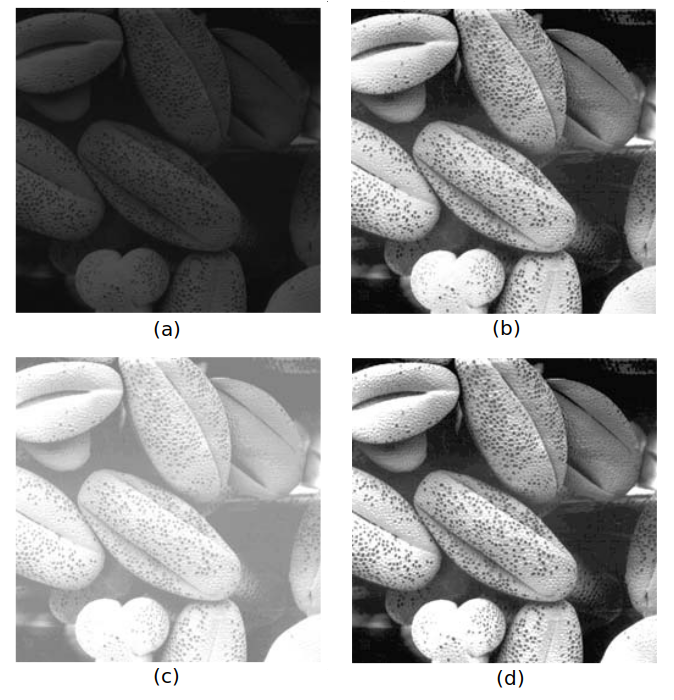
\includegraphics[scale=0.5]{images/histogram_equalization.png}
	\end{center}
	\centering
    \fadaptada{gonzalez2018digital}
\end{figure}

\subsection{Spatial Filtering}

Spatial filtering consists of the convolution of an image with a predefined kernel operator, which creates new pixel values and replaces them in the original image \cite{gonzalez2018digital}. The continuous form may be represented as a convolution over all values of a defined region of the image and the discrete form consists of sliding a weight mask over the image \cite{wu2008microscope}. Figure \ref{fig:generic_spatial_filtering} presents an arbitrary schema of a basic linear spatial filtering procedure:

\begin{figure}[htb]
	\centering
	\caption{\label{fig:generic_spatial_filtering} Arbitrary example of linear spatial filtering of an image (a) with a $3 \times 3$ filter mask (b), which results in filtered sections (c).} 
	\begin{center}
	    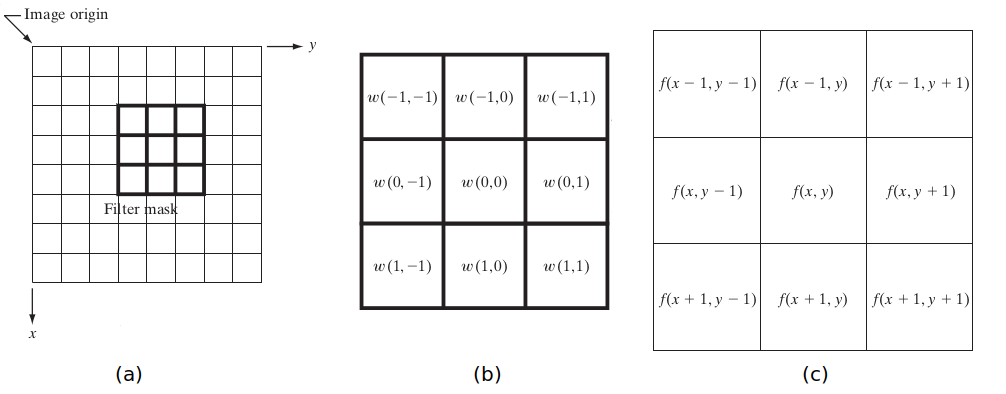
\includegraphics[scale=0.4]{images/generic_spatial_filtering.png}
	\end{center}
	\centering
    \fadaptada{gonzalez2018digital}
\end{figure}

Examples of discrete spatial filtering in digital image processing are smoothing filters, order-statistic nonlinear filters and sharpening filters, illustrated according to \cite{gonzalez2018digital}. Smoothing spatial filters are applied to remove small details, edges and lines from an image, i.e. blur, or to reduce noise. The order-statistic nonlinear filters are based on ordering pixels of the image under the filter area and replacing the pixel value in the center of the area with the response from ordering; one example is the \emph{median filter}, which replaces the center pixel with the median of pixels in its neighborhood. Median filters yield significant noise reduction effects if the nature of the noise is random. Finally, the sharpening filters are built to highlight transitions in intensity by spatial differentiation and are used for enhancing edges.

\subsection{Contrast Limited Adaptive Histogram Equalization}

Contrast enhancement may be described as the slope of the function that is relating input image intensity value to desired resultant image intensities \cite{sonali2019approach}. Histogram equalization is one of the techniques to perform contrast enhancement and works in an image by mapping the distribution of its gray levels to an approximately uniform distribution. The performance of this process is deeply related to the amount of noise in the image since it consists of peaks in the histogram, which unbalances the mapping and enhances noisy structures. One solution to this problem, according to \citeonline{zuiderveld1994constrast}, is to divide the image into \emph{contextual regions}, i.e. rectangular areas of $8 \times 8$ size, compute the optimal contrast for each of the regions and merge the results with bilinear interpolation to avoid boundary effects. This method is known as \sigla{AHE}{Adaptive Histogram Equalization}, where the global outlier gray levels do not influence each contextual region contrast enhancement.

The \sigla{CLAHE}{Contrast Limited Adaptive Histogram Equalization} method was proposed to overcome the drawback of noise. As stated by \citeonline{sonali2019approach}, it is the method that improves the low contrast issue and operates by limiting the contrast enhancement that is usually performed by ordinary histogram equalization or the AHE, which results in the noise enhancement as well. It is accomplished by allowing only a maximum number of pixels in each of the histogram bins and equally distributing the clipped pixels among the whole histogram \cite{zuiderveld1994constrast}. Figure \ref{fig:hr_ahe_clahe} presents an example of the differences between histogram equalization techniques and their results in a \sigla{MRI}{Magnetic Resonance Imaging} example:

\begin{figure}[htb]
	\caption{\label{fig:hr_ahe_clahe} MRI image of a human knee \textbf{(a)}, a simple histogram equalization \textbf{(b)}, an adaptive histogram equalization \textbf{(c)} and the contrast limited adaptive histogram equalization \textbf{(d)}.} 
	\begin{center}
	    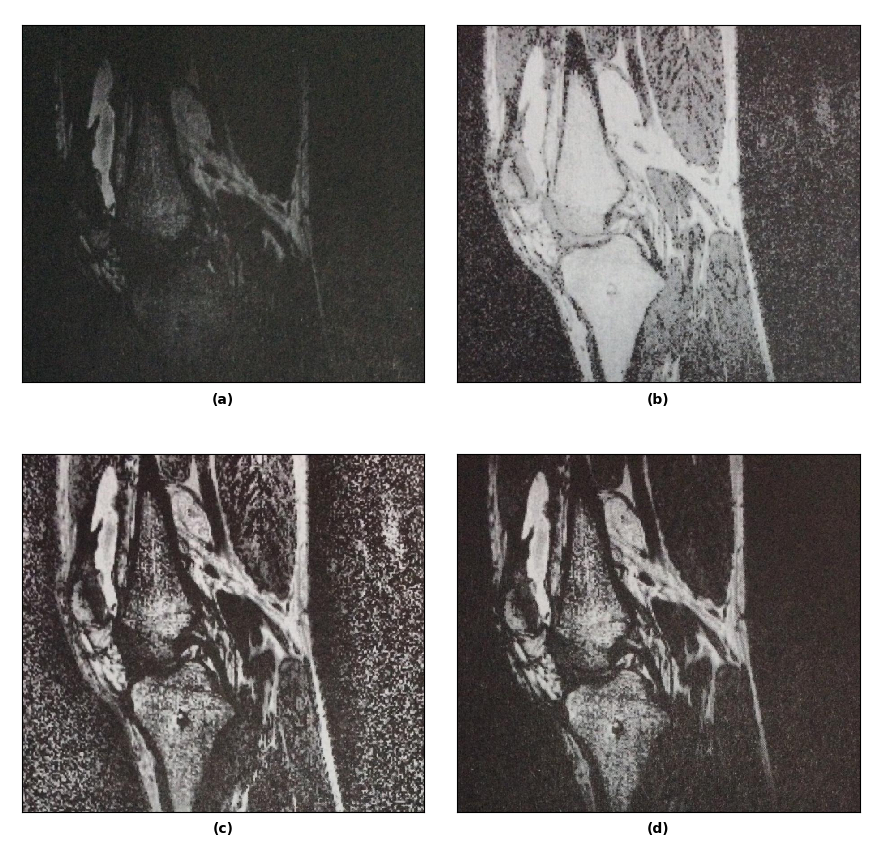
\includegraphics[scale=0.4]{images/knee_HE_AHE_CLAHE.png}
	\end{center}
	\centering
    \fadaptada{zuiderveld1994constrast}
\end{figure}
